\chapter{Self-Directed Learning}
\label{chap:sdl}

There are many ways to refer to self-directed learning (\gls{SDL}). In the middle of a definition’s diversity, I will adopt a genealogical perspective to choose an appropriate definition for \gls{SDL}. Three seminal authors are essential in this approach: Cyril Houle, Alen Tough, and Malcolm Knowles. I will explain in more detail the contributions of each of them to reach an adequate \gls{SDL} definition.

Houle’s work entitled ``Inquiring Mind'' (\citeyear{houle:1961}) introduced the first concerns that would be important to reach a future SDL concept. Brockett and Donaghy (\citeyear{brockett:2005}) narrate Houle’s study with 22 adult learners presented in this work:
\begin{citacao}
    ``He categorized these learners in three different ways based how they viewed the ‘purposes and values of continuing education’: goal-oriented, activity-oriented, and learning-oriented. It was the latter of these groups that was of particular interest relative to self-directed learning. The learning-oriented adult was described as an adult who engages in learning purely for ‘the desire to know’. Here, Houle draws parallels to self-directed learning''.
\end{citacao}

The “learning-oriented adult” category contained an incipient \gls{SDL} definition. From this context, Allen Tough and Malcolm Knowles would take important steps to a more solid definition. Tough and Knowles are former doctoral students of Houle and deepened this discussion, advancing toward a better \gls{SDL} definition. Tough (\citeyear{tough:1967}) established a similar \gls{SDL} concept as follows:
\begin{citacao}
    “When an individual decides that he wants to learn certain information, knowledge or skill, he often seeks a professional instructor to tell him how to proceed and to supervise his learning. However, instead of turning most of the responsibility over to a professional teacher, the individual may decide to act as his own teacher, and assume the primary responsibility for planning, initiating, and conducting the learning project. Such behavior can be called self-teaching and the person learning in this manner can be called a \underline{self-teacher}” (author’s emphasis).
\end{citacao}

Self-teaching was one of the first definitions to touch slightly on the \gls{SDL} concept used in this text. Some essential aspects of \gls{SDL}, like planning, initiating, and conducting the own learning, are related to this definition. Although it mentions these aspects, this definition does not have sufficient granularity regarding the main phases of the whole learning process.

At last, Knowles (\citeyear{knowles:1975}, p.~18) defined \gls{SDL} in a more specific way, covering the main phases of the learning process:
\begin{citacao}
    “In its broadest meaning, ‘self-directed learning’ describes a process in which individuals take the initiative, with or without the help of others, in diagnosing their learning needs, formulating learning goals, identifying human and material resources for learning, choosing and implementing appropriate learning strategies, and evaluating learning outcomes”.
\end{citacao}

The \gls{ISSDL} uses two definitions as references. During the 33rd \gls{ISSDL} Symposium, the \gls{ISSDL} board developed a more concise \gls{SDL} definition, “thereby helping scholars to differentiate what is and is not \gls{SDL}-related practice, research, and theory” \cite{issdl:2020}.  This definition asserts, “\gls{SDL} is an intentional learning process that is created and evaluated by the learner”. However, \gls{ISSDL} also adopts Knowles’ definition as a more extensive version. Due to the importance of the \gls{ISSDL} decision, I use Knowles’ definition as the basis for this work and the \gls{ISSDL} board’s short definition if it is necessary to refer to \gls{SDL} synthetically. I created Figure \ref{fig:sdl-process} to present the \gls{SDL} process from Knowles’ definition schematically.

\begin{figure}[ht!]
\centering

\caption{\textmd{\acrshort{SDL} process from Knowles’ definition schematically.}}
\label{fig:sdl-process}
\fcolorbox{gray}{white}{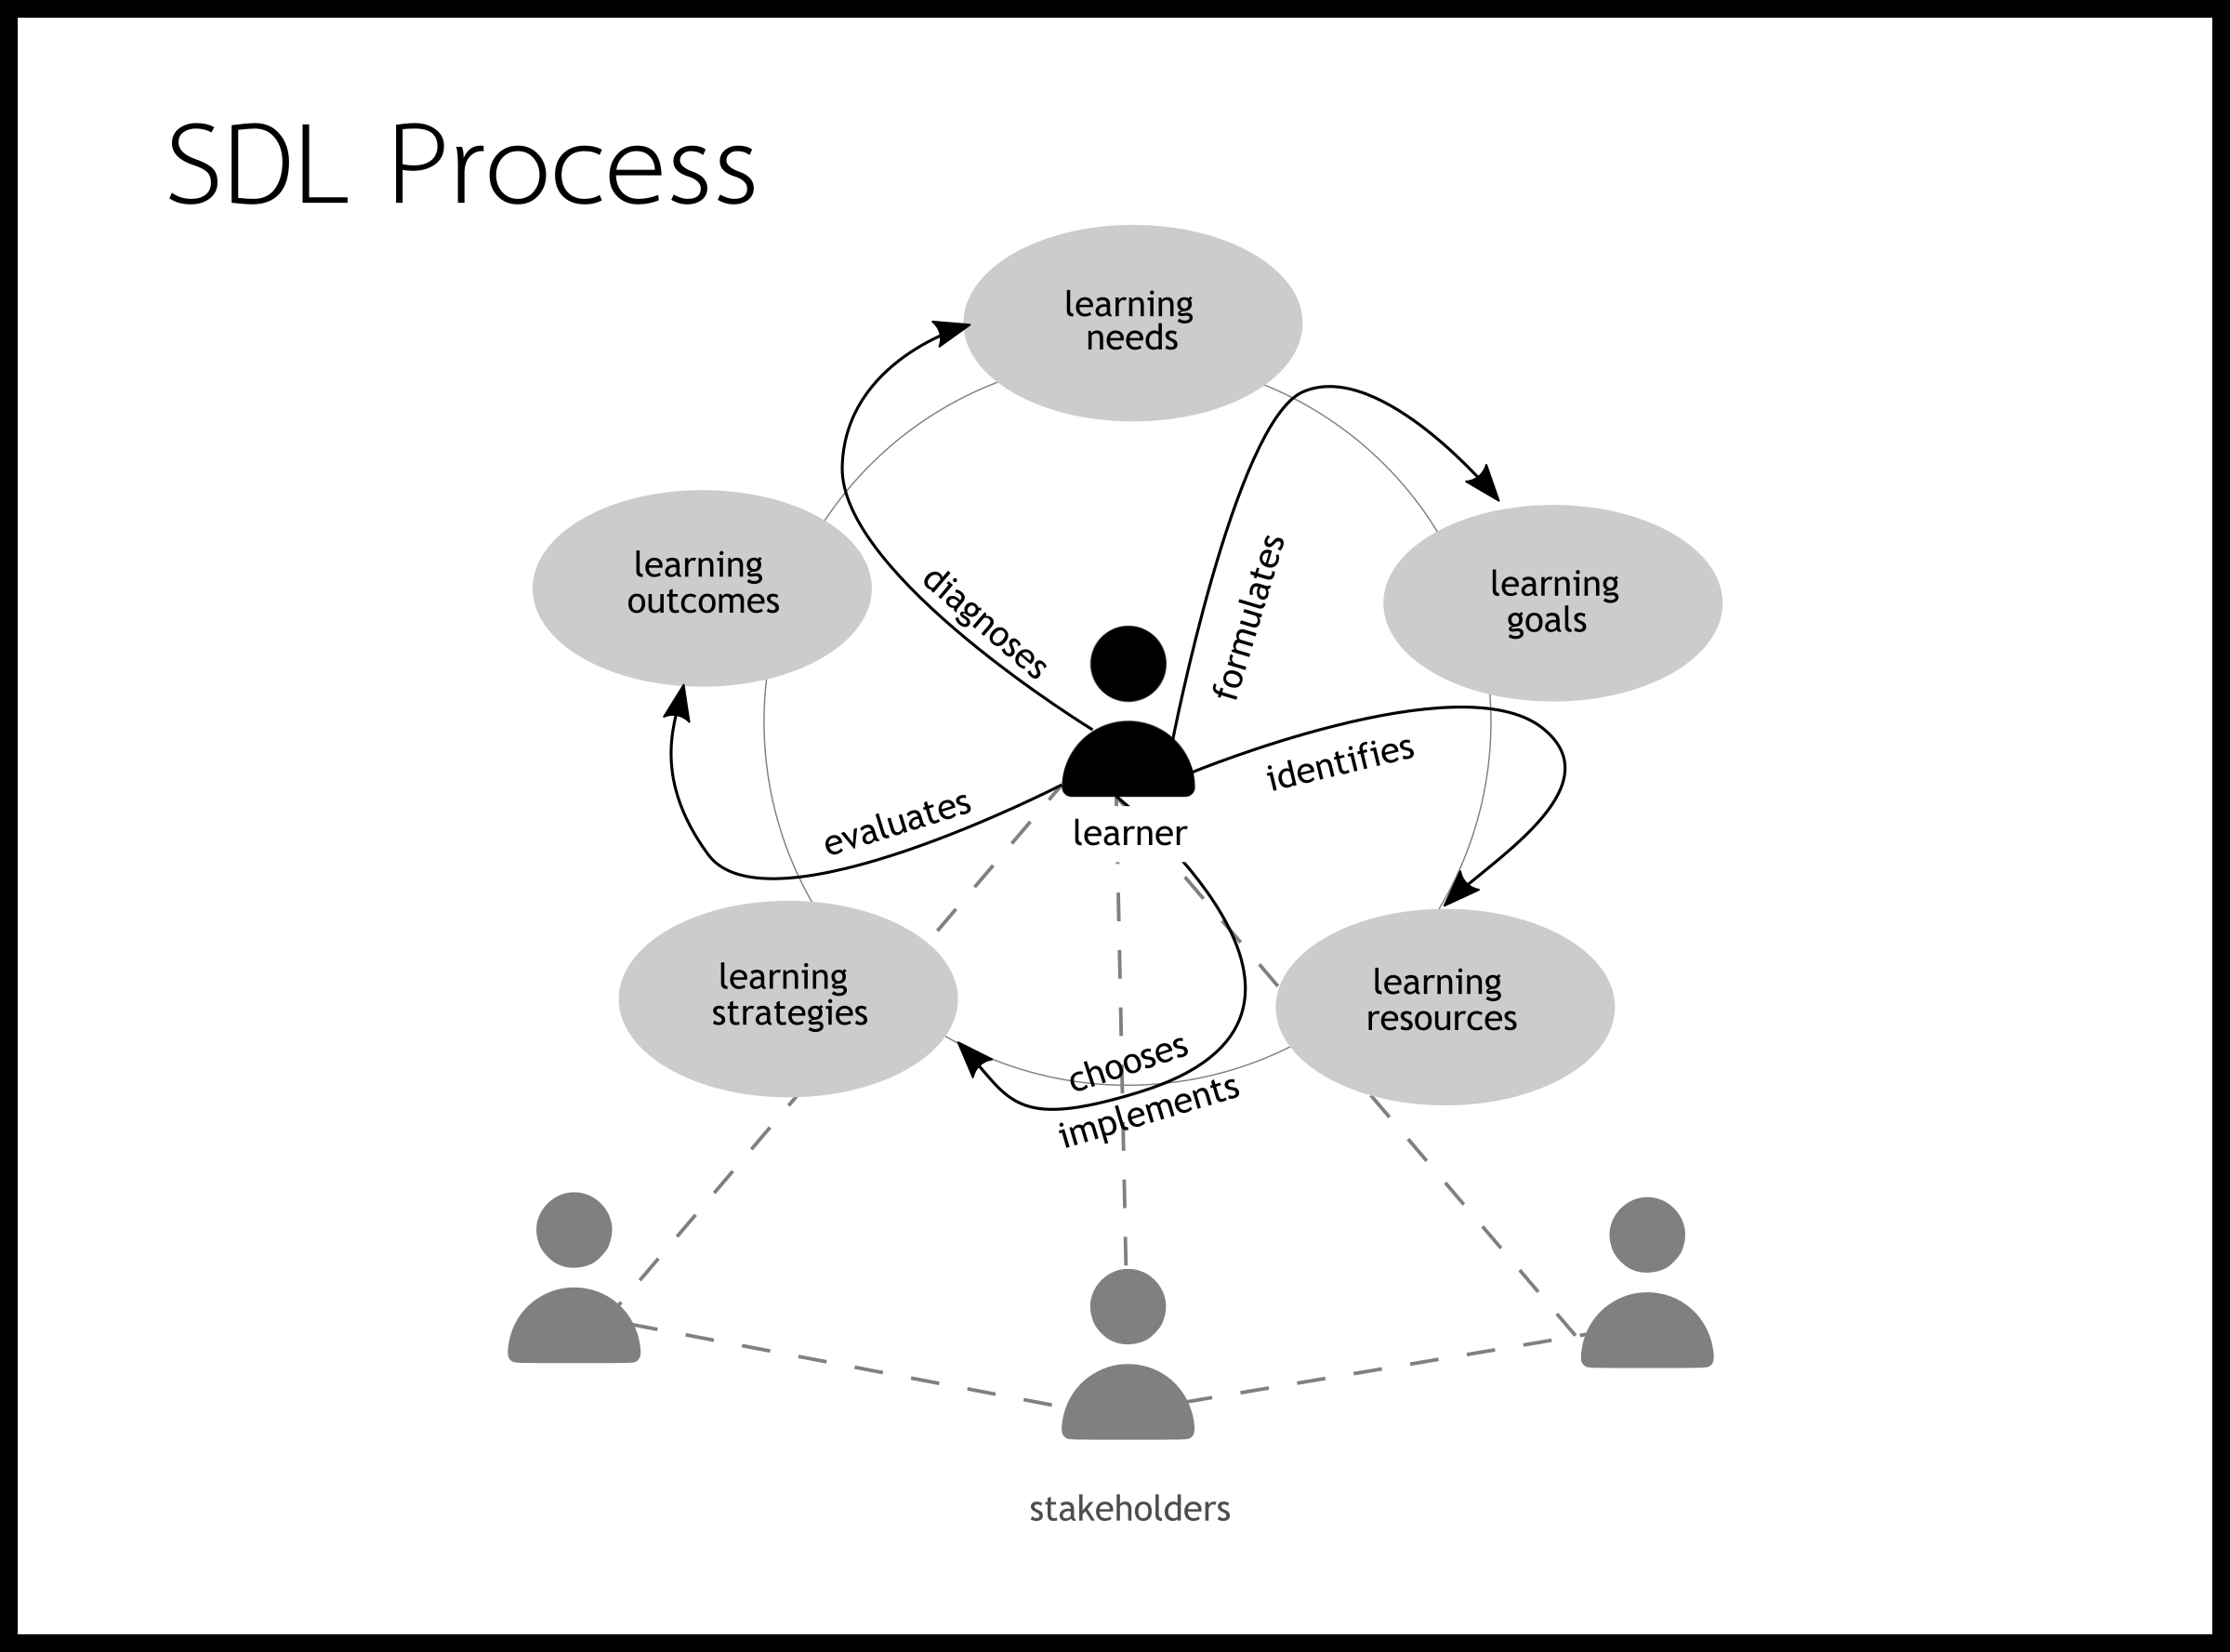
\includegraphics[width=0.9\textwidth]{images/chapter-02/sdl-process.png}}

\par\medskip\ABNTEXfontereduzida\selectfont\textbf{Source:} Created by the author (2024).
%\citeauthor{manualufpe2020} (\citeyear{manualufpe2020}) \par\medskip
\end{figure}

Throughout this chapter, I present \gls{SDL} in various aspects. Section \ref{sdl-sec:goals} points out the different \gls{SDL} goals, considering which philosophical framework the research uses as a reference. Section \ref{sdl-sec:models} enumerates the many ways to model the \gls{SDL} process, highlighting these models’ potentialities and weaknesses. Section \ref{sdl-sec:relations} establishes some relations from the \gls{SDL} concept into some approaches like andragogy, problem-based learning, and self-regulated learning. And, at last, Section \ref{sdl-sec:challenges} presents some existing research challenges involving \gls{SDL}, situating which one this research addresses.
